\newcommand\domain[3]{Let $\Omega\subseteq\reals^{#2}$, and ${#1}:\Omega \to \reals^{#3}$}
\chapter{Functions of Several Variables}
\setcounter{exercisecounter}{0}
\setcounter{thmcounter}{1}

We now relax the conditions that functions have to be linear. Moreover, we can restrict the domain of the function to be some subset $\Omega \subseteq \reals^n$, as some functions are not everywhere defined on $\reals^m$.

\example{
    Find the largest domain $\Omega\subseteq\reals^3$ such that the function \[
        f(x,y,z)=\frac{1}{x^2+y^2+z^2-9}   
    \]
    is defined.
}
The right hand side is well defined for any $x^2+y^2+z^2-9\neq 0$. That is, you can calculate the right hand side as long as you are not dividing by zero. This means we can take the largest domain to be $\Omega = \reals^3 - \{(x,y,z)|x^2+y^2+z^3=9\}$. What is this mysterious region described by $x^2+y^2+z^2=9$? Recall that $\sqrt{x^2+y^2+z^2}$ is distance of $(x,y,z)$ from the origin, so this traces out a sphere of radius $3$.

\section{Graphing in $\reals^n$}

Graphing has always been a useful tool for to gain intuition about the `shape' of functions. Here we formalize the definition of the graph of a function.

\definition{Graph}{
    \domain{f}{n}{}. We denote the \textbf{Graph} of $f$ to be $\Gamma_f$, and is the subset of $\reals^{n+1}$ \[
    \Gamma_f\defeq\{(\vec{x},f(\vec{x})) \ |\ \vec{x}\in\Omega\}.
    \]
}
Intuitively, this means we take $\Omega$ and lift that set in the $(n+1)$-st dimension according to the value of $f(\vec{x})$ evaluated at each point.
\example{
    Let $f(x,y)=(49+3x-2y)/6$, then the graph of $f$ is a plane in 3D space, which we have sketched in \hyperref[ex:1.26]{one example} in the first chapter.
}

This is not too hard to understand for one or two variables, but gets out of hand quickly as $n$ increases. I sometimes struggle to visualize even in the third dimension. One way to get around this is to look at the cross sections of a graph. 
\definition{Level set}{
    \domain{f}{n}{}. Let $c\in \reals$. The \textbf{level set} of $f$ at $c$ is denoted $L_c$, and is the set \[
    L_c\defeq \{\vec{x}\in\Omega \ | \ f(\vec{x})=c\}.
    \]
}
Why is this a natural definition? Consider the the intersection between $\Gamma_f$ and the hyperplane described by the set of $(\vec{x},c)$ for all $\vec{x}\in \reals^n$. This plane will intersect all the points in $L_c$, except they are lifted in the $(n+1)$-st dimension by $c$ units. That is, if you understand how all the $L_c$'s behave for all values of $c$, you understand how the graph of $L_c$ behaves.

\example{
    What are the level sets of the function $f(x,y)=\sqrt{x^2+y^2}$? 
}
The function here is not complicated at all: This is the distance $(x,y)$ from the origin, meaning the graph of $f$ is a cone. If we take cross section slices of positive heights, we will get circles. For negative heights, we get an empty set. For $c=0$, $L_c$ only contains the origin.

We can compress these level sets back to 2 dimensions.
\begin{figure}[h]
    \centering
    \begin{subfigure}[l]{0.46\textwidth}
    \centering
    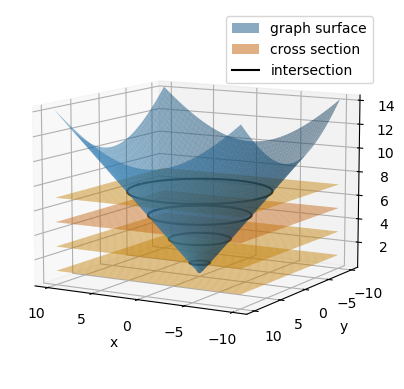
\includegraphics[width=\textwidth]{Rn_function/cone.png}
    \caption{Cross sections of the cone}
    \end{subfigure}
    \begin{subfigure}[r]{0.5\textwidth} 
        \centering
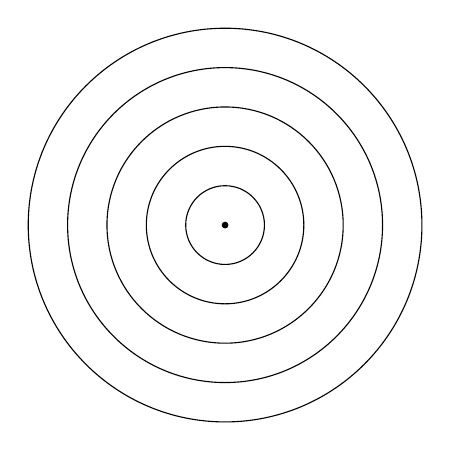
\begin{tikzpicture}
    \filldraw(0,0) circle(1pt);
    \draw (0,0)circle (0.5);
    \draw (0,0)circle (1);
    \draw (0,0)circle (1.5);
    \draw (0,0)circle (2);
    \draw (0,0) circle(2.5);
\end{tikzpicture}
\caption{The level sets $c=0$ to $c=5$, evenly spaced}.
    \end{subfigure}
\end{figure}

Let us see how our flatlander friend Frankie (apparently that is what the inhabitants of $\reals^2$ call themselves) can visualize this cone from the 2D level sets. Frankie holds a meter that constantly evaluates $f(x,y)$ at any point. He realizes that if he circles the origin at a radius of $r$, the meter will stay constant at a value of $r$. If he walks directly away from the origin, the meter will increase in value. Moreover, because the level sets $L_1,L_2,L_3,L_4,...$ are evenly spaced, Frankie only needs to walk a the same distance away from the origin to raise the meter value the same amount. Translated back to 3D, Frankie is actually `hiking' up the cone as he walks away from the origin. The slope (evaluated from the radial cross section) is $1$, so Frankie walks $k$ units away from the origin to raise his elevation by $k$, no matter where he is.

\example{
    What are the level sets of the function $f(x,y,z)={x^2+y^2+z^2}$? 
} \begin{wrapfigure}{l}{0.5\textwidth}
    \centering
    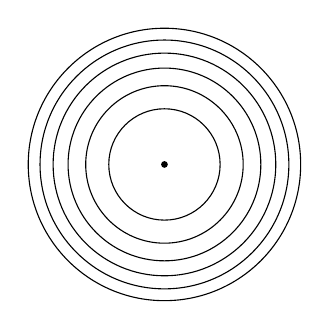
\begin{tikzpicture}
        \filldraw(0,0) circle(1pt);
        \draw (0,0)circle (0.707);
        \draw (0,0)circle (1);
        \draw (0,0)circle (1.224);
        \draw (0,0)circle (1.414);
        \draw (0,0)circle (1.58);
        \draw (0,0)circle (1.73);
    \end{tikzpicture}
    \caption{Take the 2D analog $g(x,y)=x^2+y^2$. The level sets of $c=0,1,2,\ldots$ are not evenly spaced.}
\end{wrapfigure}
Now we play the role of Frankie. 

First we try to see what the level sets $f(x,y,z)=c$ look like. This is a sphere of radius $\sqrt(c)$. The level sets are also spheres, but this time they are spaced a little bit different. To go from the level set $L_c$ to $L_{c+1}$, we go from the sphere of radius $\sqrt{c}$ to $\sqrt{c+1}$, and the shortest distance is  \begin{align*}
    \sqrt{c+1}-\sqrt{c}&=  \frac{(\sqrt{c+1}-\sqrt{c})(\sqrt{c+1}+\sqrt{c})}{(\sqrt{c+1}+\sqrt{c})}\\ &= \frac{1}{\sqrt{c+1}+\sqrt{c}}
\end{align*}

which gets smaller as $c$ increases! This means we need to walk a shorter distance to increase our meter. Equivalently, the `slope' in this direction increases as we get further away.

We could also hold $z$ constant at $0$ to take one more cross section $(x,y,0,c)$ in $x,y$. The `level sets' of the function $g(x,y)=f(x,y,0)$ look as follows:



\example{Sketch the function $f(x,y)=xy$, either in 3D or through its 2D level sets.}

Let us begin by considering the level sets $xy=c$. This describes the graph $y=c/x$, except for the case $c=0$, then the level set is the x and y axes.
\begin{figure}[h]
    \centering
    \begin{subfigure}{0.29\textwidth}
        \centering
        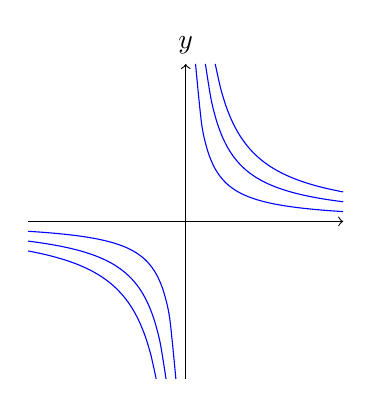
\begin{tikzpicture}[scale=0.5]
            \draw[->] (-4, 0) -- (4, 0) ;%node[right] {$x$};
            \draw[->] (0, -4) -- (0, 4) node[above] {$y$};
            %\foreach \i in {1,..,3}{
            \draw[scale=1, domain=-4:-0.25, smooth, variable=\x, blue] plot ({\x}, {1/\x});
            \draw[scale=1, domain=-4:-0.5, smooth, variable=\x, blue] plot ({\x}, {2/\x});
            \draw[scale=1, domain=-4:-0.75, smooth, variable=\x, blue] plot ({\x}, {3/\x});
            \draw[scale=1, domain=0.25:4, smooth, variable=\x, blue] plot ({\x}, {1/\x});
            \draw[scale=1, domain=0.5:4, smooth, variable=\x, blue] plot ({\x}, {2/\x});
            \draw[scale=1, domain=0.75:4, smooth, variable=\x, blue] plot ({\x}, {3/\x});
            %}
          \end{tikzpicture}
          \caption{Positive $c$}
    \end{subfigure}
    \begin{subfigure}{0.29\textwidth}
        \centering
        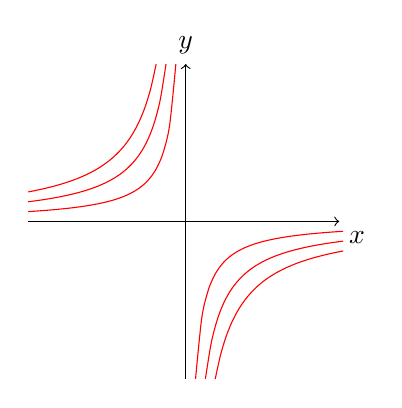
\begin{tikzpicture}[scale=0.5]
            \draw[->] (-4, 0) -- (3.9, 0) node[below right ] {$x$};
            \draw[->] (0, -4) -- (0, 4) node[above] {$y$};
            %\foreach \i in {1,..,3}{
            \draw[scale=1, domain=-4:-0.25, smooth, variable=\x, red] plot ({\x}, {-1/\x});
            \draw[scale=1, domain=-4:-0.5, smooth, variable=\x, red] plot ({\x}, {-2/\x});
            \draw[scale=1, domain=-4:-0.75, smooth, variable=\x, red] plot ({\x}, {-3/\x});
            \draw[scale=1, domain=0.25:4, smooth, variable=\x, red] plot ({\x}, {-1/\x});
            \draw[scale=1, domain=0.5:4, smooth, variable=\x, red] plot ({\x}, {-2/\x});
            \draw[scale=1, domain=0.75:4, smooth, variable=\x, red] plot ({\x}, {-3/\x});
            %}
          \end{tikzpicture}
          \caption{Negative $c$}
    \end{subfigure}
    \begin{subfigure}{0.4\textwidth}
        \centering
        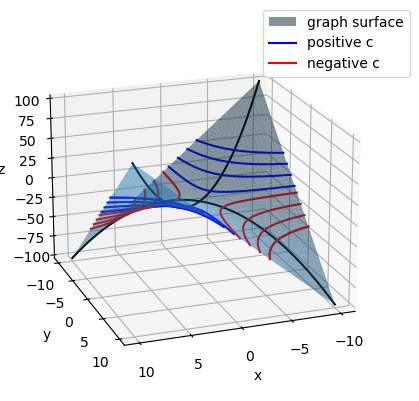
\includegraphics[width=\textwidth]{Rn_function/saddle.png}
        \caption{A saddle}
        %\caption{The surface $f(x,y)=xy$}
    \end{subfigure}
\end{figure}


 There are many ways to visualize the actual surface from here: My goto way is to vary $c$ and see how the level set changes. In this case, starting from positive $c$ and decreasing, the curves get closer and closer to the $x$ and $y$ axis, and they `flip' across the axis as the sign of $c$ changes from positive to negative.

The graph looks something like a saddle, or a pringle chip. Saddle points are somewhere between a local maximum and a local minimum. The saddle point of this function is at the origin: going the direction of $x=y$, you will get $f(x,y)=x^2$ that curves upwards; going in the direction of $x=-y$, you get $f(x,y)=-x^2$ which curves downwards. This point is \textit{in some sense} a local minimum and a local maximum depending on which way you look at it.

Indeed, we can rewrite \begin{align*}
    xy = \frac{1}{2}\left[\left(\frac{1}{\sqrt{2}}(x+y)\right)^2 - \left(\frac{1}{\sqrt{2}}(x-y)\right)^2\right],
\end{align*}
so we can rotate our basis vectors $\vec{e}_1,\vec{e}_2\in \reals^2$ to get $(\vec{e}_1-\vec{e}_2)/\sqrt{2},(\vec{e}_1+\vec{e}_2)/\sqrt{2}$. In this new basis, we can plot the rotated saddle as $(y^2 -x^2)/2$.

\begin{figure}[h]
    \centering
    \begin{subfigure}[t]{0.5\textwidth}
        \centering
        \begin{tikzpicture}[scale=0.6]
            \draw[->] (-4, 0) -- (4, 0) node[right] {$x$};
            \draw[->] (0, -4) -- (0, 4) node[above] {$y$};
            %\foreach \i in {1,..,3}{
            \draw[->] (0,0) -- (3,0) node[above]{$\vec{e}_1$};
            \draw[->] (0,0) -- (0,3) node[left]{$\vec{e}_2$};
            \draw[->,blue] (0,0) -- (2.121,2.121) node[above right]{$(\vec{e}_1+\vec{e}_2) / \sqrt{2}$};
            \draw[->,blue] (0,0) -- (2.121,-2.121) node[below right]{$(\vec{e}_1-\vec{e}_2)/\sqrt{2}$};
            %}
            \draw[->,dotted,thick] (0,3) arc (90:50:3);
            \draw[->,dotted,thick] (3,0) arc (0:-40:3);
          \end{tikzpicture}
          \caption{Positive $c$}
    \end{subfigure}
    ~
    \begin{subfigure}[t]{0.4\textwidth}
        \centering
        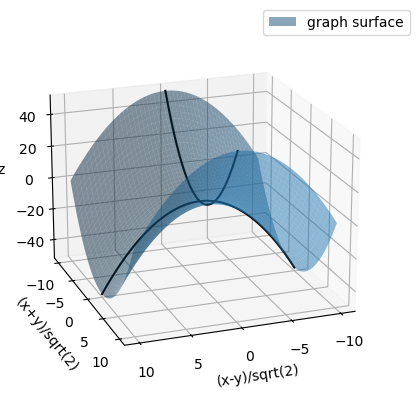
\includegraphics[width=\textwidth]{Rn_function/saddle2.png}
        \caption{The rotated saddle}
        %\caption{The surface $f(x,y)=xy$}
    \end{subfigure}
\end{figure} 
\example{Let $a,b,c>0$, and $k,m,l\in\reals$. What does the surface described by \[
    \frac{x^2-2kx}{a^2}+\frac{y^2-2my}{b^2}+\frac{z^2-2lz}{c^2}=1
\]
look like?
}
Let us approach a simplier version of the problem first: what is the surface described by \[
    \frac{x^2}{a^2}+\frac{y^2}{b^2}+\frac{z^2}{c^2}=1?
\]
We know what happens when $a=b=c=1$. Namely, we get the unit sphere. Now if we stretch the x axis by a factor of $a$, we will change from a surface \[
    x^2+y^2+z^2=1 \to \frac{x^2}{a^2}+y^2+z^2=1!
\]
Because the x,y,z axes are orthgonal, we can also stretch the y and z axes by a factor $b$ and $c$ respectively to give the surface. This will give us an ellipsoid, which is just a stretched (or compressed) sphere. To deal with the original equation, we can complete the square to get \begin{align*}
    \frac{x^2-kx}{a^2}+\frac{y^2-my}{b^2}+\frac{z^2-lz}{c^2}&=  \frac{(x-k)^2-k^2}{a^2}+\frac{(y-m)^2-m^2}{b^2}+\frac{(z-l)^2-l^2}{c^2}\\
    &=\frac{(x-k)^2}{a^2}+\frac{(y-m)^2}{b^2}+\frac{(z-l)^2}{c^2} -\frac{k^2}{a^2}-\frac{m^2}{b^2}-\frac{l^2}{c^2}, \\
\end{align*}
Which means we have an ellipsoid but now translated $(k,m,l)$ units!
In the later exercises, you will classify the surfaces described by \[
    x^2+y^2-z^2=1, \ x^2-y^2-z^2=1,
\]
which are called one and two sheeted hyperboloids respectively. 
\begin{figure}[h]
    \centering
    \begin{subfigure}[l]{0.4\textwidth}
        \centering
        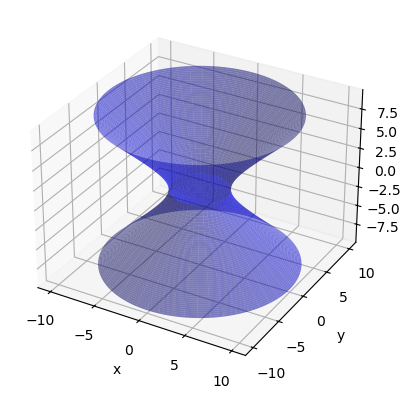
\includegraphics[scale=0.6]{Rn_function/onesheet.png}
        \caption{Hyperboloid of one sheet}
    \end{subfigure}
    \begin{subfigure}[r]{0.4\textwidth}
        \centering
        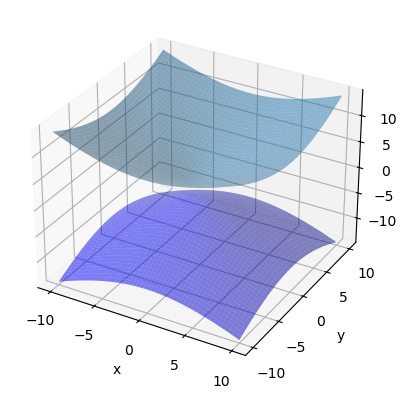
\includegraphics[scale=0.6]{Rn_function/twosheet.png}
        \caption{hyperboloid of two sheets}
    \end{subfigure}
\end{figure}
In later chapters we will see a way to change our coordinate system, through some rotation, scaling and translation, to simplify any surface in the form \[
    ax^2+by^2+cz^2+dxy+eyz+fzx+gx+hy+iz=j
\] to look like something of the form \[
    \frac{x^2}{a^2}\pm\frac{y^2}{b^2}\pm\frac{z^2}{c^2}
\]
\exercises
\begin{exerciselist}
    \item Consider the level set $x^2+y^2-z^2=1$. \begin{enumerate}[label=(\alph*)]
        \item We take the cross section of this surface with the plane $z=k$. What does this cross section look like in $x,y$?
        \item We now hold $y=0$. What does this cross section look like?
        \item Combine the first two parts, and try to sketch the surface in 3D. How many sheets or `connected regions' does this hyperboloid have?
    \end{enumerate}
    \item Consider the level set $x^2-y^2-z^2=1$. \begin{enumerate}[label=(\alph*)]
        \item We take the cross section of this surface with the plane $x=k$. What does this cross section look like in $y,z$? How does this part differ from the last problem?
        \item We now hold $y=0$. What does this cross section look like?
        \item Combine the first two parts, and try to sketch the surface in 3D. How many sheets or 'connected regions' does this hyperboloid have?
    \end{enumerate}
    \item What the largest possible domain for the function \begin{enumerate}[label=(\alph*)]
        \item $f(x,y)=e^{x^2-y^2}$
        \item $f(x,y)=\ln (y^2-x^2-2)$
        \item $f(x,y)=(x^2-y^2)/(x-y)$
        \item $f(x,y,z)=1/(xyz)$
        \item $f(x,y,z)=(z^2-x^2-y^2)^{-1/2}$.
    \end{enumerate}
    \item Describe the graph of the function \begin{enumerate}[label=(\alph*)]
        \item $f(x,y)=5$
        \item $f(x,y)=2x-y$
        \item $f(x,y)=1-x^2-y^2$
        \item $f(x,y,z)=4-\sqrt{x^2+y^2}$
        \item $f(x,y,z)=\sqrt{24-4x^2-6y^2}$.
    \end{enumerate}
    \item Describe the level sets of the function \begin{enumerate}[label=(\alph*)]
        \item $f(x,y)=x+y$
        \item $f(x,y)=x^2+9y^2$
        \item $f(x,y)=x-y^2$
        \item $f(x,y)=x-y^3$
        \item $f(x,y)=x^2+4x+y^2+2y+9$
        \item $f(x,y,z)=x^2+y^2-z$
        \item $f(x,y,z)=x^2+2x+y^2-2y+z^2+4z$
        \item $f(x,y,z)=z^2-x^2-y^2$
    \end{enumerate}
    \item Describe the surfaces in $\reals^3$ described by $f(x,y,z)=$ \begin{enumerate}[label=(\alph*)]
        \item $x^2+y^2=16$
        \item $z^2=49x^2+y^2$
        \item $z=25-x^2-y^2$
        \item $x=4y^2-z^2$
        \item $4x^2+y^2+9z^2=36$
        \item $4x^2-y^2+9z^2=36$
        \item $4x^2-y^2-9z^2=36$
    \end{enumerate}
    \item Let $c\in \reals$. Describe the intersection of the graph of $f(x,y)=x^2+9y^2$ in the given planes $x=c$, $y=c$, $z=c$.
    \item \todo Intersection of cone with plane is a circle
\end{exerciselist}
\section{Topology of $\reals^n$}
\begin{remark}[Author's notes]
    This part is slightly touched on in Even's textbook (but scattered across the differentiation chapter). Some past 281 instructors such as John Enns dedicate half a week on topology.  
\end{remark}
\definition{Open Ball}{
    Let $\vec{x}_0\in\reals^n,r>0$. We write the \textbf{open ball of radius $r$ centered at $a$} as $B(\vec{x}_0,r)$, and is the set of all points within $r$ distance away from $a$, i.e. \[
    B(\vec{x}_0,r)\defeq \{x\in\reals^n \ | \ |\vec{x}-\vec{x}_o|<r\}.
    \]
}
    Many statements that we will work towards are `local', in the sense that they only dependent on the behavior of a function in a small open ball centered at a point. For instance, if a function $f:\reals\to\reals$ is continuous at $x=0$, altering the value of the function at any $y\neq 0$ will not change the continuity of the function at $x=0$. This is because the function remains unchanged in the small open ball $B(0,|y|/2)$. Similar, the differentiability (and its derivative) also only depends on the local behavior of the function.

    Thus, we define a set with a special property that each point in the set is `fully contained' inside the set.

\definition{Open sets}{
    Let $\Omega\subseteq \reals^n$.
    We say that $\Omega$ is \textbf{open} if for every $\vec{x}\in\Omega$, there is some radius $r_{\vec{x}}>0$ 
such that $B(\vec{x},r_{\vec{x}})\subseteq\Omega$.}
\begin{remark}
    We want to deal with open sets when we talk about the local behavior of a function. It is not useful to talk about the continuity of a function that is only defined on the integers, this set is not open because every ball centered at an integer will contain a non-integer.
\end{remark}
\proposition{An open ball is open.}
Yeah, this needs a proof.
To show this is open, let $\vec{x} \in B(\vec{x}_0,r)$. Our goal is construct a value $r_{\vec{x}}>0$ such that $B(\vec{x},r_{\vec{x}})\subseteq B(\vec{x}_0,r)$.

\begin{wrapfigure}{l}{0.6\textwidth}
    \centering
    \begin{tikzpicture}
        \node [label=right:{$\vec{x}_0$}] at(0,0) {\textbullet} ;
        \draw [dotted] (0,0) circle (3);
        \draw (0,0)--(-3,0) node [midway, below] {$r$}; 
        \node [label=right:{$\vec{x}$}]at (1.5,1.5) {\textbullet};
        \draw [dotted,red,thick] (1.5,1.5) circle (0.879);
        \draw [thick, red] (1.5,1.5)--(0.878,2.1215) node [midway, left] {$r_{\vec{x}}$}; 
    \end{tikzpicture}
\end{wrapfigure}
As long as the distance between $\vec{x}$ and $\vec{x}_0$ is strictly less than $r$, the points within a small vicinity of $\vec{x}$ all have distance $<r$ to $\vec{x}_0$.

This can be made rigorous using the Triangle Inequality.
\begin{proof}
    Let $\vec{x} \in B(\vec{x}_0,r)$. Let $r_{\vec{x}}= r-|\vec{x}_0-\vec{x}|$. Then for any $\vec{y}\in B(\vec{x},r_{\vec{x}})$, we have\begin{align*}
        |\vec{y}-\vec{x}_0|&= |\vec{y}-\vec{x}+\vec{x}-\vec{x}_0|\\ &\leq |\vec{y}-\vec{x}|+|\vec{x}-\vec{x}_0| \\& < r-|\vec{x}_0-\vec{x}|+|\vec{x}_0-\vec{x}|\\& =r,
    \end{align*}
   
    so $\vec{y}\in B(\vec{x}_0,r)\implies B(\vec{x},r_{\vec{x}})\subseteq B(\vec{x}_0,r)$.
\end{proof} \ \\
\example{
    The following sets are open:
    \begin{enumerate}
        \item The top-half plane in $\reals^2$. $\mathbb{H}\defeq \{(x,y) \ | \ y>0\}$. Sketch: for every $(x,y)\in\mathbb{H}$ take $r_{(x,y)}=y$.
        \item The punctured ball $B^*(\vec{x},r)\defeq B(\vec{x},r)-\{\vec{x}\}$. Sketch: for every $\vec{y}\in B^*(\vec{x},r)$ take $r_{\vec{y}}=\min(|\vec{y}-\vec{x}|, r-|\vec{y}-\vec{x}|)$.
        \item The whole space $\reals^n$ is open. Sketch: take $r_{\vec{x}}=1$ for any point.
        \item The union of (possibly infinite) open sets $\bigcup_a G_a$, where each $G_a$ is open. Sketch: if $\vec{x}\in \bigcup_a G_a$, then $\vec{x}\in G_a$ for some $a$. Because $G_a$ is open, pick a radius such that the ball is contained in $G_a$.
    \end{enumerate}
    The following sets are not open:
    \begin{enumerate}
        \item The set contianing just one point $\{\vec{x}\}$. Sketch: every ball centered at $\vec{x}$ contains points outside of $\vec{x}$.
        \item The set of points $\{\vec{x}\in \reals^n \ | \ |\vec{x}|\leq r\}$. Sketch: Any ball of radius $\epsilon>0$ centered around the point $(r,0,0,\ldots, 0)$ contains $(r+\epsilon,0,0,\ldots,0)$.
    \end{enumerate}
}
We see that a set fails to be open if there is a point in the boundary of the set. I.e. no matter how small $\epsilon>0$ is, $B(\vec{x},\epsilon)$ extends beyond that set.
\definition{Boundary}{
    Let $\Omega\subseteq\reals^n$. We denote the \textbf{boundary} of $\Omega$ as $\partial \Omega$. This is the set of points in $\vec{x}\in\reals^n$ such that every open ball around $\vec{x}$ contains a point in $\Omega$ and a point not in $\Omega$.
}
Colloquially, $\vec{x}$ is very (arbitrarily) close to $\Omega$, but is also very (arbitrarily) close to $\Omega^c$. So it is on the boundary of the two sets.

\example{
    In $\reals^3$, $\partial B(\vec{0},r)$ is the sphere of radius $r$. Note that a sphere refers to only the surface while a ball consists of the whole interior.
}
\definition{Closure of a set and Closed sets}{
    Let $\Omega\subseteq\reals^n$. We denote the \textbf{closure of $\Omega$} as $\bar{\Omega}\defeq \Omega\cup \partial\Omega$. If $\bar{\Omega}=\Omega$, we say $\Omega$ is \textbf{closed}. Equivalently, a set is closed if it contains its boundary.
}
\proposition{The closure of a set is closed.}
What this means is that if we add in the boundary of a set, we do not create new `boundaries'.
\begin{proof}
    Let $\Omega\subseteq \reals^n$. Let $\vec{x}\in \partial \bar{\Omega}$. Consider open ball of radius $\epsilon>0$ centered around $\vec{x}$. We want to show that this ball contains a point in $\Omega$ and a point in $\partial \Omega$, thus $\vec{x}\in\partial \Omega$ so is already included in $\bar{\Omega}$. 
    
    This ball, by the definition of boundary of $\bar{\Omega}$, contains a point $\vec{a}\in\bar{\Omega}$ and a point in $\vec{b}\in\bar{\Omega}^c$. We first consider $\vec{b}$. Because $\vec{b}\in\bar{\Omega}^c\subseteq (\Omega \cup \partial\Omega)^c = \Omega^c \cap (\partial\Omega)^c\subseteq \Omega^c$. This point is in $\Omega^c$ too.
    If $\vec{a}\in \Omega$, we are done. Else, $\vec{a}\in\partial \Omega$. As $B(\vec{x},\epsilon)$ is open, we can find some open ball $B(\vec{a},\delta)\subseteq B(\vec{x},\epsilon)$. Now we can reapply the definition for $\vec{a}\in\partial \Omega$ to get that there is some point $\vec{a}'\in B(\vec{a},\delta)$ that is in $\Omega$. So we have some $\vec{a}'\in B(\vec{x},\epsilon)$ that is contained in $\Omega$.

    Since $\epsilon$ was arbitrary, we can conlude that every open ball centered around $\vec{x}$ contains a point in $\Omega$ and $\Omega^c$. So $\vec{x}\in\partial \Omega\subseteq \bar{\Omega}$.
\end{proof}

\exercises
\begin{exerciselist}
    \item \todo
\end{exerciselist}
\section{Limits and Continuity}
\definition{Limit Point}{
    Let $\Omega\subseteq\reals^n$. A \textbf{limit point of $\Omega$} $\vec{x}\in\reals^n$ is a point such that every open ball centered around $\vec{x}$ contains a point $\vec{y}\in\Omega$ with $\vec{y}\neq \vec{x}$. Alternatively, using the notation of punctured balls $B^*(\vec{x},r)\defeq B(\vec{x},r)-\{\vec{x}\}$, the intersection \[
        B^*(\vec{x},r)\cap\Omega
    \] is non-empty for every $r>0$.
}
Colloquially, you can approach (get closer and closer to) a limit point by using only points in $\Omega$.
\begin{remark}
    When we talk about limits, we care about the behavior around some point $\vec{x}$ but not at the point $\vec{x}$ (For all we care about, $\vec{x}$ could be outside the domain of the function). This is why the condition $\vec{y}\neq\vec{x}$ is in the definition of a limit point.
\end{remark}
\definition{Limit}{
    \domain{f}{n}{m}. Let $\vec{a}$ be a limit point of $\Omega$, $\vec{b}\in\reals^m$. We denote \textbf{the limit of $f(\vec{x})$ as $\vec{x}$ tends to $\vec{a}$} as $\lim_{\vec{x}\to\vec{a}}$, and say that this limit equals $\vec{b}$ if for all $\epsilon>0$, there is $\delta>0$ such that \[
    |f(\vec{x})-\vec{b}|<\epsilon \textrm{ if } \vec{x}\in B^*(\vec{x},\delta)\cap \Omega,
    \]
    or equivalently, \[
        |f(\vec{x})-\vec{b}|<\epsilon \textrm{ if } 0<|\vec{x}-\vec{a}|<\delta
    \]
    where $f$ is defined.
}
\subsubsection*{Parsing the $\epsilon-\delta$ definition of limit}
For an illustration. Let $\Omega=\reals^2$ and $f:\reals^2\to\reals^2$. We want to consider the limit \[
\lim_{\vec{x}\to\vec{0}}f(\vec{x})=\vec{b}.
\]
We draw the function as taking in values from the input space $\reals^2$ and spitting them them out in the output space $\reals^2$.  
\begin{figure}[h]
    \centering
        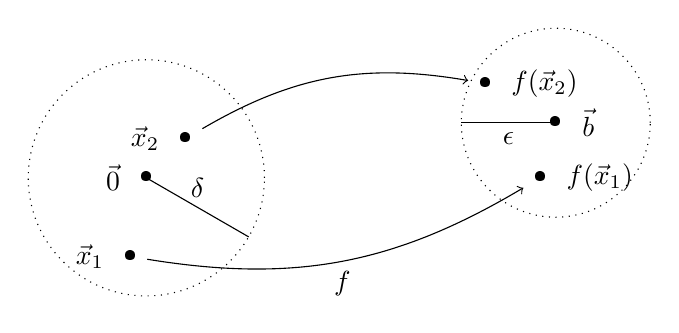
\begin{tikzpicture}
            \node (A) [label=left:{$\vec{x}_1$}]at(-.2,-1) {\textbullet};
            \node (ori) [label=left:{$\vec{0}$}]at(0,0) {\textbullet};
            \node(C) [label=left:{$\vec{x}_2$}] at (0.5,0.5) {\textbullet};
            \node(D)[label=right:{$f(\vec{x}_2)$}]
            at (4.3,1.2) {\textbullet};
            \draw[->](C) edge[bend left =20] (D);
        \node (B) [label=right:{$f(\vec{x}_1)$}]at (5,0) {\textbullet};
    \draw[->] (A) edge [bend right=20]  node[midway, below]{$f$} (B);
    \draw [dotted] (ori) circle (1.5);
    \draw (0,0)--(1.3,-0.75) node[midway, above]{$\delta$}; 
    \node (lim) [label=right:{$\vec{b}$}] at (5.2,0.7){\textbullet};
        \draw [dotted](lim) circle (1.2);
        \draw (5.2,0.7) -- (4,0.7) node[midway, below] {$\epsilon$};
        
    \end{tikzpicture}
\end{figure}

We do not know what the value $f(\vec{0})$ is - it may not exist. However, we can see if the surrounding values of $f$ approaches some value. To make this rigorous, let's say we want to get within $\epsilon$ distance of the value $\vec{b}$. This corresponds to the open ball on the right. Now we want to pick $\delta$ such that at a very short distance $\delta$ away from $\vec{0}$, the image of $B^*(\vec{0},\delta)$ lands within $B(\vec{b},\epsilon)$. This corresponds to the left open ball.

That means, you can get as close as you like to $\vec{b}$ as long as you are close to $\vec{0}$. If the $\epsilon$ requirement for closeness changes from $0.1$ to $0.0000001$, you can just pick a smaller $\delta$ to get within this distance. Remember: the order of the limit is someone first challenges that you need to get close to the limit in the output space ($\epsilon$), then you pick the ball around the input space ($\delta$) that satisfies that particular value of $\epsilon$.

\proposition{
    Suppose $\lim_{\vec{x}\to\vec{a}}f(\vec{x})$ exists, then it must be unique.
}
\begin{proof}
    Suppose, for the sake of contradiction, we have the two limits $\vec{b}\neq\vec{b}'$ of $f$ as $\vec{x}\to\vec{a}$. Let $\epsilon=|\vec{b}-\vec{b}'|$. Pick $\delta_1,\delta_2$ such that $|f(\vec{x})-\vec{b}|<\epsilon$ and $|f(\vec{x}-\vec{b}'|<\epsilon|$ when $0<|\vec{x}-\vec{a}|<\delta_1$ and $0<|\vec{x}-\vec{a}|<\delta_2$ respectively. Then pick some $\vec{x}$ such that $0<|\vec{x}-\vec{a}|<\min(\delta_1,\delta_2)$. For this particular value of $\vec{x}$,\[
        \epsilon=|\vec{b}'-\vec{b}|= |\vec{b}'-f(\vec{x})+f(\vec{x})-\vec{b}|\leq|\vec{b}'-f(\vec{x})|+|\vec{b}-f(\vec{x})| <\frac{\epsilon}{2}+\frac{\epsilon}{2}=\epsilon.
    \]
    This gives us the strict inequality $\epsilon<\epsilon$, which is impossible.
\end{proof}
\begin{remark}
    A consequence of this is that if a limit exists, the limit will be the same using any path of approach. Caution: It is not enough to check a few paths to confirm a limit exists. Take the function \[
        f(x,y)=\begin{cases}
            1 &\textrm { if } x=0\\
            0 &\textrm{otherwise }
        \end{cases}
    \]
    Approaching $f(0,0)$ along any straight line $y=cx$ will give a limit of $0$. However, the limit does not exist, as approaching on the y-axis $x=0$ will give a limit of $1$. 
\end{remark}
\example{
    Compute the limit (if it exists) of \[
    \lim_{(x,y)\to (0,0)} \frac{xy}{\sqrt{x^2+y^2}}
    \]
}
Let's assume that this limit exists, what must it be? We can test the limit along the x-axis and y-axis. I.e. We set $x$ or $y=0$ and let the the other variable approach $0$. If the limit exists, the limit should be the same no matter how which axis we approach the limit by. Then we see \begin{align*}
    (x=0) \lim_{y\to 0}\frac{0y}{\sqrt{0+y^2}}& =0 \\
    (y=0)\lim_{x\to 0}\frac{0x}{\sqrt{x^2+0}}&=0
\end{align*}
So the limit, if it exists, must be $0$.
Can we show that this exists? Let $\epsilon>0$, then $\delta=[\textrm{placeholder}]$. We want \begin{align*}
    \left|\frac{xy}{\sqrt{x^2+y^2}}-0\right|<\epsilon
\end{align*} whenever $\sqrt{x^2+y^2}<\delta$. Intuitively, this should be true as the degree of the numerator is $2$ and the degree of the denominator is `$1$'. So the numerator shrinks to $0$ much faster than the denominator. To make this rigorous, we can use the inequality $|x|=\sqrt{x^2}\leq \sqrt{x^2+y^2}$ and similarly, $|y|\leq \sqrt{x^2+y^2}$ to get \[
    \left|\frac{xy}{\sqrt{x^2+y^2}}-0\right|\leq\left|\frac{x^2+y^2}{\sqrt{x^2+y^2}}\right|
    =\left|\sqrt{x^2+y^2}\right|<\delta.
\]
So setting $\delta=\epsilon$ works! Now we just replace the placeholder with $\epsilon$ and pretend we knew this all along.
\begin{proof}
    We claim the limit is $0$. Let $\epsilon>0$, then for all $|(x,y)|<\epsilon$, we have  \[
        \left|\frac{xy}{\sqrt{x^2+y^2}}-0\right|\leq\left|\frac{x^2+y^2}{\sqrt{x^2+y^2}}\right|
        =\left|\sqrt{x^2+y^2}\right|<\epsilon.
    \]
\end{proof}
\example{
    Compute the limit (if it exists) of \[
    \lim_{(x,y)\to(0,0)} \frac{2x^2+y^2}{x^2+y^2}.
    \]
}
Again, we test a few paths to approach this limit to see what it can be.
Approaching from the y-axis $x=0$, we get \[
\lim_{y=0}\frac{y^2}{y^2}=\lim_{y=0}1 =1.
\]
But if we approach from the x-axis $y=0$, we will get\[
    \lim_{x=0}\frac{2x^2}{x^2}=\lim_{x=0}2 =2.
\]
These two limits are not equal, so we can conclude that the limit does not exist.



